\chapter{Graphs and paths}




\section{Graphs}


\subsection{Overview}
A (directed) graph is a set of nodes and each node has a list of pointers to their neighbour nodes. You can use such a graph for path finding - within your scene there's a graph with way nodes and possible directed ways between them, meaning that there may be cases you can go from node A to node B, but not from B to A - then for instance a \emph{find the shortest way from node A to node D} query can be performed on this graph and you will receive a path with a list of nodes you have to pass if you want to walk from the source to the target node. HOW you find this source and target graph nodes in another story... for this, you need to find the graph node which is nearest to your source world position, the same for the target. You can do this by iterating over ALL graph nodes and finding the closest graph node, or by using some kind of hierarchy to make this task more performant...

All different graphs are managed like textures, meshes etc. through a manager and resource handlers. The graph manager is accessed through \emph{GraphManager::GetInstance()}.

Here's an example how such a graph may look like:

\begin{lstlisting}[caption=Graph example]
Test graph:                  Shortest paths: ('source'->
                             'target' = nodes to pass)

+------5------+              A->A = A
|             |              A->B = A->B
|  /-2--B--3--C--5-\         A->C = A->D->C
| /     |    /|     \        A->D = A->D
+-A     2 /3/ 1      F       A->E = A->D->E
  \     |/    |     /        A->F = A->D->E->F
   \-1--D--1--E--2-/

\end{lstlisting}

Normally for path finding, only the \emph{distances} between the nodes are taken into account - not their \emph{real} positions within the world.



\subsection{File format}
PixelLight graph files have the extension \emph{graph}.

Note that the distance attribute of a neighbour node is optional, if this attribute is not given or has a negative value, the distance is calculated automatically. Normally you can ignore this distance attribute - manipulate it only for special tasks by hand!





\section{Paths}



\subsection{Overview}
A path consists of a set of nodes at different world coordinates. An actor can for example move along this path automatically. If the path is closed which can be set using the \emph{GraphPath} function \emph{SetClosed()}, actors will move to the first node if the last one was reached.

The most important path function is \emph{GetPosByNodeIndex()} which will return the path world position at a given time. The first parameter is the node index were 1.5 will be between two nodes. With the second parameter you can define whether the position is interpolated in a linear and rough way or if you want to receive positions which lies on a smooth curve. If the position isn't linear interpolated the first and last node are skipped because they will be used to define the behaviour of the curve.

Here's an example how such a path may look like:

\begin{lstlisting}[caption=Path example]
  /B-------------C\
 /                 \
A                   D
 \                 /
  \F-------------E/
\end{lstlisting}

An actor can be moved along a path for example in the way shown below:

\begin{lstlisting}[caption=Moving along path]
fTimer += PLCore::Timing::GetInstance()->GetTimeDifference();
pMyActor->SetPosition(pMyPath->GetPosByNodeIndex(fTimer));
\end{lstlisting}

Normally you only use a simple timer to move on the path. The example above shows the simplest way to move an actor along a path, this isn't useful if you also want to perform e.g. collision detection. In this way you should use the path points only as \emph{move to} targets were the actor should try to move to and then working with for instance forces to the target.

\begin{figure}
  \begin{center}
    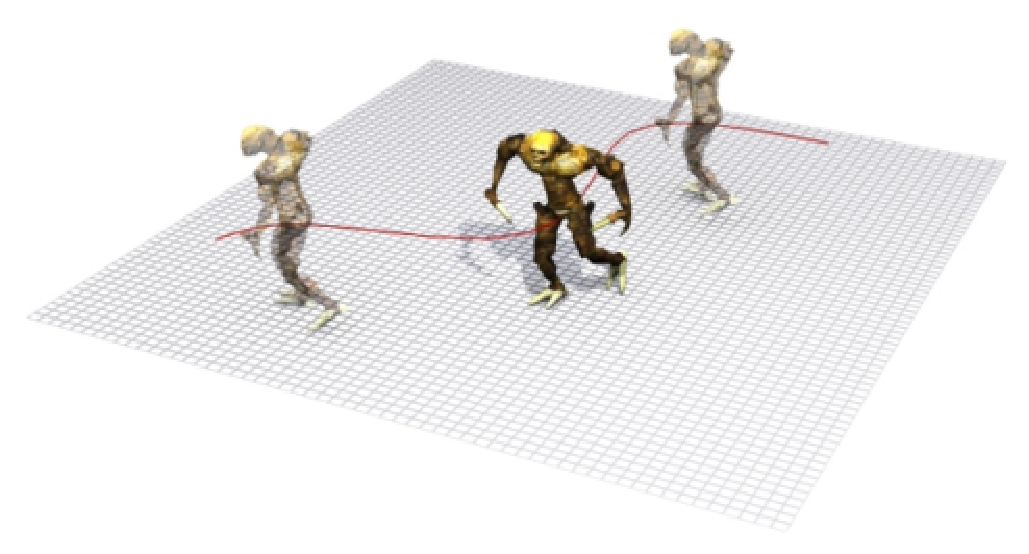
\includegraphics{pics/Paths.eps}
  \end{center}
  \caption{Actor walking on a path}
  \label{fig:Actor walking on a path}
\end{figure}

Paths can be build by hand or automatically as result of for instance a graph query. (path finding)


\subsection{Create paths by hand}
It's possible to build a path by hand during runtime. Call the graph path managers creation function \emph{GraphPathManager::Create()} to generate a new path. The function will return a pointer to the new path and now it's up to you to fill up this path with nodes.

New nodes are added using the path function \emph{GraphPath::AddNode()} which will take a path node as parameter. Note that this path node is just linked. The path node itself is in the simplest case only a world coordinate. \emph{GraphNode} also offers some tool functions like to compute the distance to another node using \emph{GetDistance()}.

Example:

\begin{lstlisting}[caption=Path creation example]
//	Test path:
//	  /B-------------C\
//	 /                 \
//	A                   D
//	 \                 /
//	  \F-------------E/

// Build path visualized above
GraphPath cPath;
GraphNode *pNode;

// A
pNode = new GraphNode("A");
cPath.AddNode(*pNode);
pNode->SetPos(0.0f, 0.0f, 2.0f);
// B
pNode = new GraphNode("B");
cPath.AddNode(*pNode);
pNode->SetPos(2.0f, 0.0f, 0.0f);
// C
pNode = new GraphNode("C");
cPath.AddNode(*pNode);
pNode->SetPos(16.0f, 0.0f, 0.0f);
// D
pNode = new GraphNode("D");
cPath.AddNode(*pNode);
pNode->SetPos(19.0f, 0.0f, 2.0f);
// E
pNode = new GraphNode("E");
cPath.AddNode(*pNode);
pNode->SetPos(16.0f, 0.0f, 4.0f);
// F
pNode = new GraphNode("F");
cPath.AddNode(*pNode);
pNode->SetPos(2.0f, 0.0f, 4.0f);

// The path should be closed
cPath.SetClosed(true);
\end{lstlisting}


\subsection{File format}
PixelLight path files have the extension \emph{path}.
